\section{Exploring Univariate Distributions in R}

\subsection{Histograms}

One of the most common ways to examine a the distribution of
observations for a single variable is to use a histogram. The
\lstinline!hist()! function creates simple histograms in R.

\begin{R}
> hist(turtles$length) # create histogram with fxn defaults
> ?hist # check out the documentation on hist
\end{R}
Note that by default the \lstinline!hist()! function plots the
frequencies in each bin. If you want the probability densities instead
set the argument \lstinline!freq=FALSE!.
%
\begin{R}
> hist(turtles$length,freq=F) # y-axis gives probability density
\end{R}
Here's some other ways to fine tune a histogram in R.

\begin{R}
> hist(turtles$length, breaks=12) # use 12 bins
> mybreaks = seq(85,185,8)
> hist(turtles$length, breaks=mybreaks) # specify bin boundaries
> hist(turtles$length, breaks=mybreaks, col='red') # fill the bins with red
\end{R}

\subsection{Density Plots}

One of the problems with histograms is that they can be very sensitive
to the size of the bins and the break points used. This is due to the
discretization inherent in a histogram. A `density plot' or `density
trace' is a continuous estimate of a probability distribution from a set
of observations. Because it is continuous it doesn't suffer from the
same sensitivity to bin sizes and break points. One way to think about a
density plot is as the histogram you'd get if you averaged many
individual histograms each with slightly different breakpoints.
%
\begin{R}
> d <- density(turtles$length)
> plot(d)
\end{R}
%
A density plot isn't entirely parameter free -- the parameter you should
be most aware of is the `smoothing bandwidth'.

\begin{R}
> d <- density(turtles$length) # let R pick the bandwidth
> plot(d,ylim=c(0,0.020)) # gives ourselves some extra headroom on y-axis
> d2 <- density(turtles$length, bw=5) # specify bandwidth
> lines(d2, col='red') # use lines to draw over previous plot
\end{R}
The bandwidth determines the standard deviation of the `kernel' that is
used to calculate the density plot. There are a number of different
types of kernels you can use; a Gaussian kernel is the R default and is
the most common choice. See the documentation for more info.

The \lstinline!lattice! package is an R library that makes it easier to
create graphics that show conditional distributions. Here's how to
create a simple density plot using the \lstinline!lattice! package.

\begin{R}
> library(lattice)
> densityplot(turtles$length) # densityplot defined in lattice
\end{R}
Notice how by default the \lstinline!lattice! package also drew points
representing the observations along the x-axis. These points have been
`jittered' meaning they've been randomly shifted by a small amount so
that overlapping points don't completely hide each other. We could have
produced a similar plot, without the lattice package, as so:

\begin{R}
> d <- density(turtles$length)
> plot(d)
> nobs <- length(turtles$length)
> points(jitter(turtles$length), rep(0,nobs))
\end{R}
Notice that in our version we only jittered the points along the x-axis.
You can also combine a histogram and density trace, like so:

\begin{R}
> hist(turtles$length, 10, xlab='Carapace Length (mm)',freq=F)
> d <- density(turtles$length)
> lines(d, col='red', lwd=2) # red lines, with pixel width 2
\end{R}
Notice the use of the \lstinline!freq=F! argument to scale the histogram
bars in terms of probability density.

Finally, let's some of the features of \lstinline!lattice! to produce
density plots for the `length' variable of the turtle data set,
conditional on sex of the specimen.

\begin{R}
> densityplot(~length | sex, data = turtles)
\end{R}
There are a number of new concepts here. The first is that we used what
is called a `formula' to specify what to plot. In this case the formula
can be read as `length conditional on sex'. We'll be using formulas in
several other contexts and we discuss them at greater length below. The
\lstinline!data! argument allows us to specify a data frame or list so
that we don't always have to write arguments like
\lstinline!turtles$length! or \lstinline!turtles$sex! which can get a
bit tedious.

\subsection{Box Plots}

Another common tool for depicting a univariate distribution is a `box
plot' (sometimes called a box-and-whisker plot). A standard box plot
depicts five useful features of a set of observations: the median
(center most line), the upper and lower quartiles (top and bottom of the
box), and the minimum and maximum observations (ends of the whiskers).

\begin{figure}[htbp]
\centering
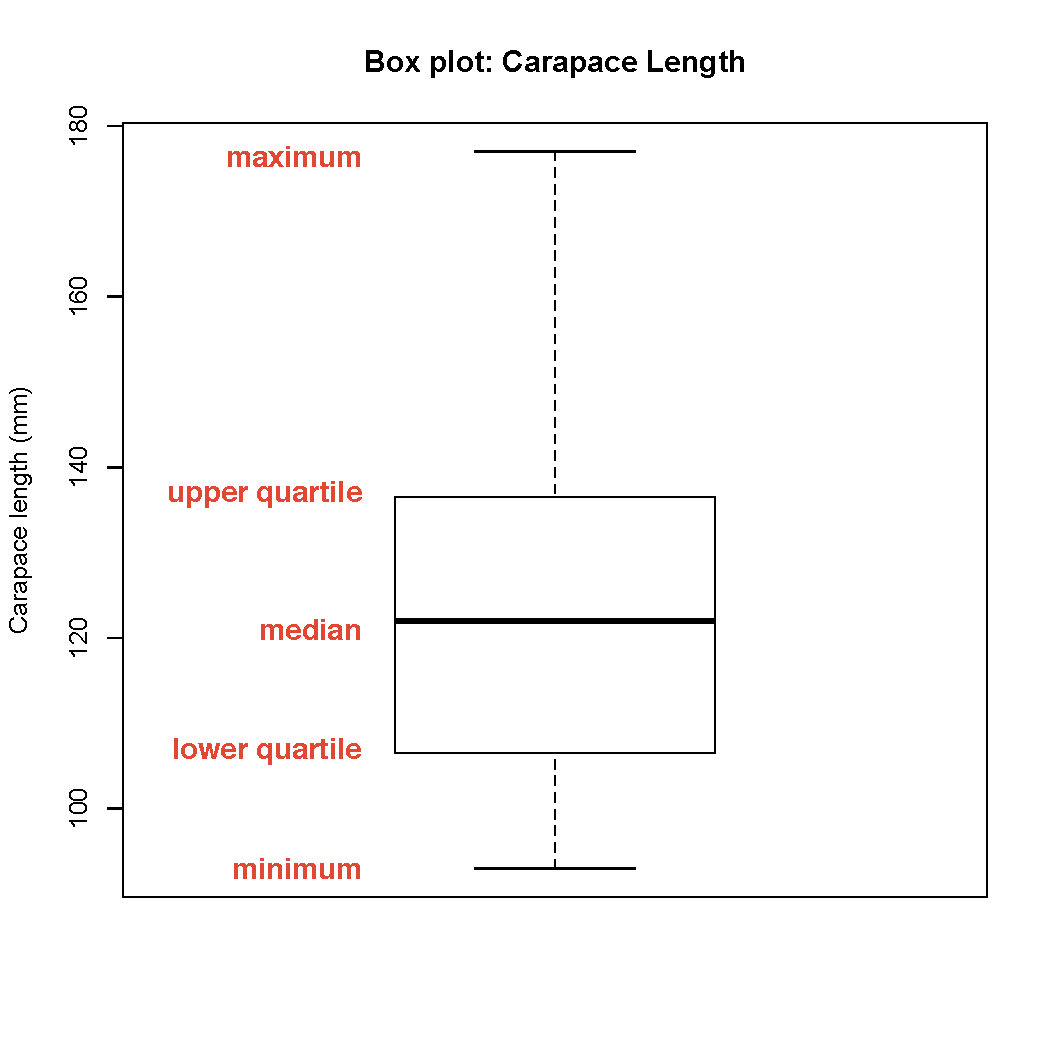
\includegraphics[width=0.5\columnwidth]{./figures/hands-on2/boxplot-labeled.pdf}
\caption{A box plot represents a five number summary of a set of
observations.}
\end{figure}

There are many variants on box plots, particularly with respect to the
`whiskers'. It's always a good idea to be explicit about what a box plot
you've created depicts.

Here's how to create box plots using the standard R functions as well as
the lattice package:

\begin{R}
> boxplot(turtles$length)
> boxplot(turtles$length, col='darkred', horizontal=T) # horizontal version
> title(main = 'Box plot: Carapace Length', ylab = 'Carapace length (mm)')
> bwplot(~length,data=turtles) # using the bwplot function from lattice
\end{R}
Note how we used the \lstinline!title()! function to change the axis
labels and add a plot title.

\paragraph{Historical note}

-- The box plot is one of many inventions of the statistician John W.
Tukey. Tukey made many contributions to the field of statistics and
computer science, particularly in the areas of graphical representations
of data and exploratory data analysis.

\subsection{Bean Plots}

My personal favorite way to depict univariate distributions is called a
`beanplot'. Beanplots combine features of density plots and boxplots and
provide information rich graphical summaries of single variables. The
standard features in a beanplot include the individual observations
(depicted as lines), the density trace estimated from the observations,
the mean of the observations, and in the case of multiple beanplots an
overall mean.

\begin{figure}[htbp]
\centering
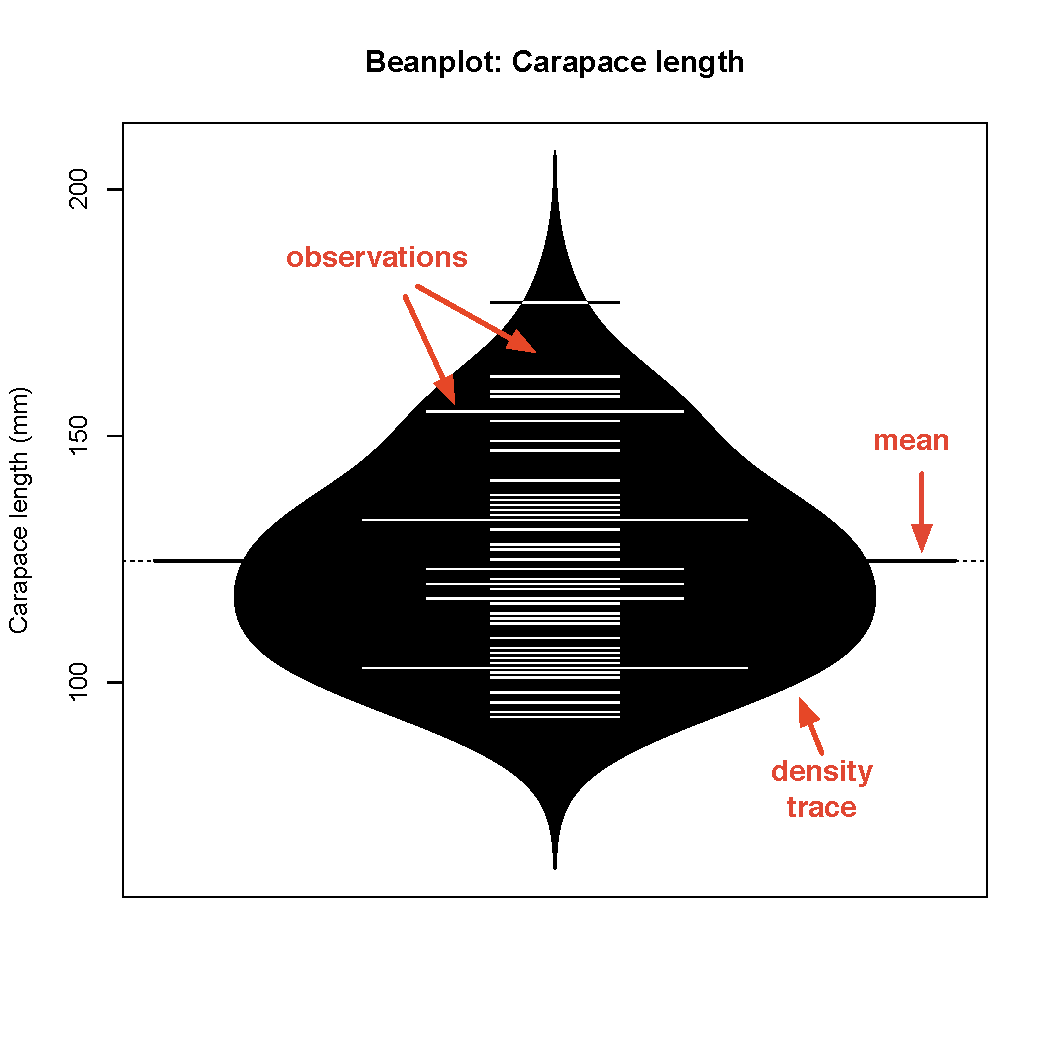
\includegraphics[width=0.5\columnwidth]{./figures/hands-on2/beanplot-labeled.pdf}
\caption{Beanplots combine features of density and box plots.}
\end{figure}

The \lstinline!beanplot! package is not installed by default. To
download it and install it use the R package installer under the
\lstinline!Packages & Data! menu (standard R GUI) or in
\lstinline!Tools > Install Packages...! in RStudio (see also the
\lstinline!Packages! tab in the lower-right window in RStudio). If this
is the first time you use the package installer you'll have to choose a
CRAN repository from which to download package info (I recommend you
pick one in the US). Once you've done so you can search for `beanplot'
from the Package Installer window. You should also check the 'install
dependencies' check box.

Once the beanplot package has been installed check out the examples to
see some of the capabilities:

\begin{R}
> library(beanplot)
> example(beanplot)
\end{R}
If you ran the examples in RStudio, use the \lstinline!Clear All! option
in the \lstinline!Plots! tab after running the examples in order to
reset parameters that the examples changed.

Note the use of the \lstinline!library()! function to make the functions
in the \lstinline!beanplot! library available for use. Here's some
examples of using the \lstinline!beanplot! function with the turtle data
set:

\begin{R}
> beanplot(turtles$length) # note the message about log='y'
> beanplot(turtles$length, log='') # DON'T do the automatic log transform
> beanplot(turtles$length, log='', col=c('white','blue','blue','red'))
\end{R}
In the final version we specified colors for the parts of the beanplot.
See the explanation of the \lstinline!col! argument int he beanplot
function for details.

We can also compare the carapace length variable for male and female
turtles.

\begin{R}
> beanplot(length ~ sex, data = turtles, col=list(c('red'),c('black')),
names = c('females','males'),xlab='Sex', ylab='Caparace length (mm)')
\end{R}
Note the use of the formula notation to compare the carapace length
variable for males and females. There is also a asymmetrical version of
the beanplot which can be used to more directly compare distributions
between two groups. We explore this below. Note too the use of the list
argument to \lstinline!col!, and the use of vectors within the list to
specify the colors for female and male beanplots.

We can also create a beanplot with multiple variables in the same plot
if the variables are measured on the same scale.

\begin{R}
> beanplot(turtles$length, turtles$width, turtles$height, log='',
names=c('length','width','height'), ylab='carapace dimensions (mm)')
\end{R}
